\subsection{Referring expression generation}
\label{sec:referring-expression-generation-game}
\subsubsection*{Setup}

In a next step, it is tested if the agents can learn to extract features of the objects together.
For this the same sender as in the previous section is used.
Based on the results, $h_s$ is fixed to $500$ and $e_s$ to $100$
However, the task and by that the receiver's architecture is adapted in two different ways.
In the first setup, the \textbf{referring expression generator}, the receiver is tasked to describe the target object with natural language following the \emph{incremental GRE-algorithm} based on the sender's message (see Figure \ref{fig:caption_generator_game_architecture}).
This follows the approach of the approach of the \emph{RE generators} described in section \ref{sec:referring_expression_generation}.
The whole scene is encoded using the \emph{image encoder} submodule, projecting it to the image encoding dimension $e_{ri}=100$.
The sender's message is decoded with the hidden size $h_r=500$ and $e_r=100$, and concatenated with the encoded image.
This is then reduced to $LSTM_o=1500$ dimensions based on the results of the previous experiments, and used as the initial state of the captioning LSTM.
Tokens are embedded with $LSTM_e=15$ dimensions.
Since the position of the padding as well as the order of the words in the target didn't have an effect on the results, the usual approach in natural generation task is used: padding tokens are appended and the referring expression is not reversed.
During training, the ground truth caption is used as the input to the LSTM using teacher forcing.
% SD: I'm not sure how teacher forcing is implemented, see my earlier comment
% DK: typo, teacher forcing is actually applied (done)
When presented with test data, the LSTM always produces three tokens, by using its own predicted words as the input for the next step.
The loss is calculated using cross entropy.

\begin{figure}[ht]
    \centering
    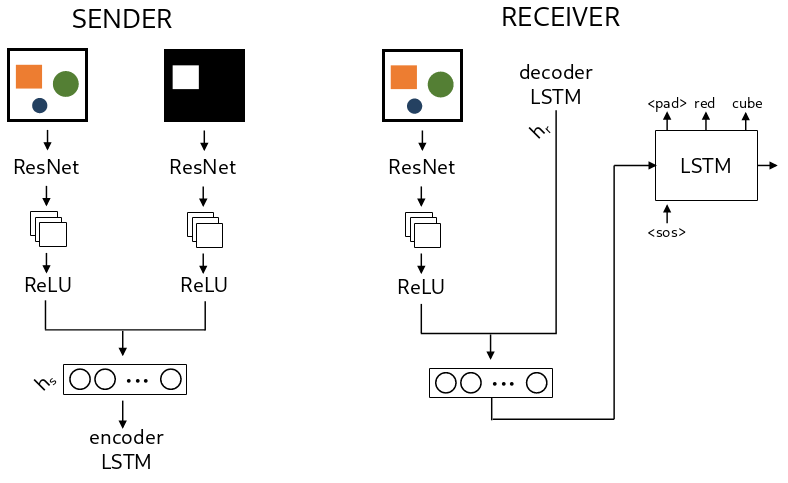
\includegraphics[width=.7\linewidth]{figures/arch_caption_generator_game.png}
    \caption{Simplified architecture of the caption generator game}
    \label{fig:caption_generator_game_architecture}
    % SD: But here we don't need an LSTM, we just want to identify one of the objects. The LSTM should only encode the inout message.
    % DK: TODO
\end{figure}

However, this setup could lead to two problems:
First, the task is quite complex for both agents to learn, since two language generation steps are involved.
This might stop the agents from converging towards a useful language.
Secondly, in case a language emerges, it could be aligned with the natural language of the target referring expressions.
In other words, the sender might just learn to effectively repeat the target referring expressions without extracting the necessary features themselves.
For that reason, in the second setup the receiver is tasked to predict only the attributes of the target object in the shape of a one-hot vector.
By this, no natural language including its salience order is involved and the complexity of the complete game is reduced.
The receiver uses the same way to encode and combine the complete scene and the sender's message with $e_{ri}=100$, $h_r=500$ and $e_r=100$.
This is then passed to a linear layer that produces a vector with 13 dimension, corresponding to the 2 sizes, 3 shapes, and 8 colors.
The loss is then calculated using binary cross entropy.

\cmtDK[inline]{figure}

The experiments for both setups are conducted with a learning rate of $2\times10^{-4}$.
As in the previous section, the following values for the variables are compared:
\begin{itemize}
    \item $|V|$: 2, 10, 16, 50, 100
    \item $n$: 1, 2, 3, 4, 6
\end{itemize}

Since the agents are trained to describe the target object discriminatively based on the described GRE-algorithm, they are trained on the \emph{Dale-2}, \emph{Dale-5} and \emph{CLEVR color} dataset.
The \emph{Dale-5} and the \emph{CLEVR color} should be again much harder to learn, since there are more objects that the agents need to discriminate the target object from.
% SD: So the sender is generating descriptions following the GRE policy?
% DK: TODO
The same metrics as in the section \ref{sec:referring_expression_generation} are used to evaluate the results for the first setup.
When predicting one-hot vectors, an overall \textbf{accuracy} is reported that reflects if all attributes were predicted correctly.
Additionally, the accuracy for each attribute is calculated separately to show which attributes give bigger challenges for the models.

\subsubsection*{Results}
\begin{table}[ht]
    \centering
    \begin{tabular}{ccc|ccc|ccc}
        \toprule
              &         &         & \multicolumn{3}{c}{\textbf{Dale-2}} & \multicolumn{3}{c}{\textbf{Dale-5}}                                                                             \\\cmidrule(lr){4-6}\cmidrule(lr){7-9}
        $|V|$ & $h_{s}$ & $h_{r}$ & \textbf{Acc.}                       & \textbf{word-by-word}               & \textbf{length} & \textbf{Acc.} & \textbf{word-by-word} & \textbf{length} \\\midrule
        {10}  & {10}    & {10}    & {22,9\%}                            & {62,8\%}                            & {1}             & {7,1\%}       & {40\%}                & {1}             \\
        {13}  & {10}    & {10}    & {22,8\%}                            & {62,9\%}                            & {0}             & {7,3\%}       & {38,7\%}              & {1}             \\
        {20}  & {10}    & {10}    & {24,6\%}                            & {64\%}                              & {1}             & {6,7\%}       & {38,7\%}              & {1}             \\
        {100} & {10}    & {10}    & {24,4\%}                            & {62\%}                              & {1}             & {7,8\%}       & {40\%}                & {1}             \\
        {100} & {100}   & {100}   & {21\%}                              & {62\%}                              & {1}             & {6,5\%}       & {37,8\%}              & {1}             \\
        \bottomrule
    \end{tabular}
    \caption{Results of the caption generator: $|V|$ are different vocabulary sizes and $h$ hidden sizes.}
    % SD: What is word-by-word?
    % DK: the same as in the caption generator with a single model (QUESTION)
    \label{tab:results_caption_generator_game}
\end{table}

The results of the caption generator game are summarized in Table \ref{tab:results_caption_generator_game}.
In general, it can be seen that the agents have much bigger problems, to solve the task together than a single neural network.
The highest accuracy for descriptions, the agents manage to predict correctly is at 24,6\% for images of the 'Dale-2' dataset.
Compared to the (masked) accuracy of the single model with 72\%, the agents predict 47,4\% points less correct descriptions.
A similar worse performance can be seen for the 'Dale-5' dataset.
Here, the agents only manage to produce for 7,8\% of the images correct descriptions with a vocabulary size of 100, 13,2\% points less than the single neural model.
The same effect can be seen for the word-by-word accuracy, which is much lower than the metric for the single neural model for both datasets.
% SD: With the vocabulary size of 100.
% DK: (done)

When looking, how the different variables affect the performance, it can be seen that a bigger vocabulary size tends to help the agents.
% SD: Not sure. The difference is still very small, within a couple of %.
% DK: TODO
This is only visible for the 'Dale-2' dataset.
With constant hidden sizes of 10, the agents score around 22,9\% with only 10 and 13 available symbols.
When this is increased to 20 and respectively 100 symbols, the agents can increase their accuracy to around 24,5\%.
However, the increase is relatively small.
Interestingly, this effect only occurs, when the hidden sizes are small with only 10 dimensions.
As soon as they are increased to 100 dimensions with a vocabulary size of 100 symbols, the accuracy drops to 21\%.
% SD: Very small decerase for such a large difference in vocabulary size compared to what we have seen earlier.
% DK: TODO

Looking at the 'Dale-5' dataset, the increase is still there, when the vocabulary is increased to 100 symbols.
Nonetheless, the difference is with 0,5\% points even smaller and the reason may be due to other influences, such as the random initialization of the weights of the agents.
This is confirmed, when looking at emerged languages.
In all the setups, the same message is communicated for all samples, independently of the input image.
This is also reflected in the length of the messages.
For the setup with a vocabulary size of $|V| = 13$, no message is transferred, and the accuracy stays the same as in the other setups.
% SD: Here it would be much better to have a loss curve to show differences in loss between the number of communication events, the same could also be done for accuracy. Then we would have a clearer picture of how vocabulary size affects learning. It could be that with 100 vocabulary there is actually a better performance than before the final cut-off point. Is this possible? How was the final cut-off point determined anyway?
% DK: TODO

These results show that the agents are not at all able to encode meaning about the images and target objects in their messages.
% SD: Negative result: how can we then interpret that? What could we change? What did we learn from this?
% DK: TODO
This is especially interesting, compared to single model caption generator in section \ref{sec:referring_expression_generation}.
In these experiments, the model was able to converge towards correct captions and therefore able to extract the necessary information.
This shows that a main challenge for the agents lies in grounding symbols in these extracted features.
